\chapter{الإيكولوجيا السلوكية}\label{ch:b3:behavioural-ecology}

يقف السرقاط على تلّ نمل أبيض بينما تحفر بقية جماعته عن
الطعام، فإذا ظهر صقر نبح فاندفع الآخرون إلى جحورهم. وقد قضى
الحارس ساعة لا يأكل وجعل نفسه أظهر حيوان في الصحراء. فلماذا؟
والطاووس يجرّ ذنبًا يكلفه خُمس ميزانية طاقته ويبطئ فراره من
النمور. ونحلة عسل عائدة من حقل ترقص على قرص عمودي، وزاوية
رقصتها إلى الشاقول هي زاوية الطعام إلى الشمس. وقرقف كبير
يصطاد اليرقات في رقعة من الأوراق يغادرها وفيها يرقات لم
تُوجد بعد. ولم يقرأ أي من هذه الحيوانات هذا الفصل، ومع ذلك
يسلك كل واحد كأنه حلّ مسألة أمثلة، أو لعبة، أو مسألة في
محاسبة القرابة. والإيكولوجيا السلوكية دراسة السلوك مجموعةَ
حلول متطورة: فيمَ السلوك، من حيث المورّثات التي ينشرها، وما
الذي يجب أن تكون عليه كلفه وفوائده حتى ينتجه الانتخاب
الطبيعي. وأدواتها أدوات الاقتصادي --- الأمثلة، \omterm{prop:b3:behavioural-ecology:hawk-dove}{ونظرية
الألعاب}، ومحاسبة القرابة --- ومحكّها الميدان.

\section{أربعة أسئلة وآلة الغريزة}

\begin{definition}[أسئلة تينبرغن]\label{def:b3:behavioural-ecology:tinbergen}
\index{أسئلة تينبرغن الأربعة}\index{نمط فعل ثابت}\index{منبّه إشاري}\index{انطباع}\index{فترة حرجة}
قال تينبرغن (1963) إن الوصف التام لأي سلوك يجب أن يجيب عن
أربعة أسئلة: \emph{آليته} (أي المنبّهات والآلة العصبية التي
تنتجه)، و\emph{نماؤه} (كيف ينشأ في الفرد، من المورّثات
والخبرة)، و\emph{وظيفته} (كيف يسهم في البقاء والتكاثر)،
و\emph{تاريخه التطوري} (كيف نشأ من سلوك سلفي). وقد أرسى
علماء السلوك الذين صاغوها الأولين. وكثير من السلوكات
\emph{أنماط فعل ثابتة}: متواليات نمطية يطلقها \emph{منبّه
إشاري} بسيط وتجري إلى تمامها متى بدأت --- فإوزة رمادية تدحرج
بيضةً مزاحة راجعةً إلى العش بمنقارها، وتتم الحركة حتى لو
أُزيلت البيضة في منتصفها؛ وفرخ نورس الرنجة ينقر بقعة حمراء
على أي شيء بشكل منقار، وينقر عصًا بثلاثة أشرطة حمر أكثر مما
ينقر رأس نورس حقيقي؛ وذكر شوكة الظهر يهاجم أي شيء أحمر من
أسفله، بما في ذلك عربة بريد مارّة تُرى من النافذة. وسلوكات
أخرى تُتعلَّم ضمن نافذة: و\emph{الانطباع}، الذي يجعل فرخ
الإوزة في يومه الأول يتبع ما يتحرك ويعامله بعد ذلك والدًا ---
إوزةً، أو لورنتس، أو صندوق ورق مقوّى --- سريع لا رجعة فيه
محصور في \emph{فترة حرجة}؛ وتعلم الغناء في الطيور، وهو مثال
مجلد السنة الثانية، على الشكل نفسه. والتقابل بين الفطري
والمتعلَّم زائف: فللسلوك برنامج وراثي يحدد ما يُتعلَّم، ومتى،
وممن، والبرنامج هو ما يتطور.
\end{definition}

\begin{proof}[شواهد]
أرست تجارب تينبرغن الميدانية المنهج. فالزنابير الحفارة
(\emph{Philanthus}) ترجع إلى عش مخبأ في الرمل؛ فحرّك حلقةً من
أكواز الصنوبر كان قد وضعها حول أحد المداخل بينما كانت
الزنبورة غائبة، فبحثت في مركز الحلقة المزاحة --- فقد كانت قد
تعلمت المعالم. والنوارس السوداء الرؤوس تزيل قشور البيض من
العش بعد الفقس؛ فوضع بيضًا بجانب قشور مطلية وقشور طبيعية
وأشياء أخرى، وعدّ ما أخذته الغربان: فقد اجتذب السطحُ الأبيض
الداخلي للقشرة المفترسات، وكانت الإزالة التي بدت نظافةً
تمويهًا. وقد قاست تجارب فراخ النوارس منبّهًا إشاريًا بعرض
رؤوس من ورق مقوّى تتباين في سمة واحدة في كل مرة. وتبعت إوزُّ
لورنتس المنطبعةُ عليه مدى حياتها؛ وانطبع بط في يومه الأول
على صندوق متحرك فلم يمكن بعدها أن يُجعل يتبع بطة.
\end{proof}

\begin{omfigure}
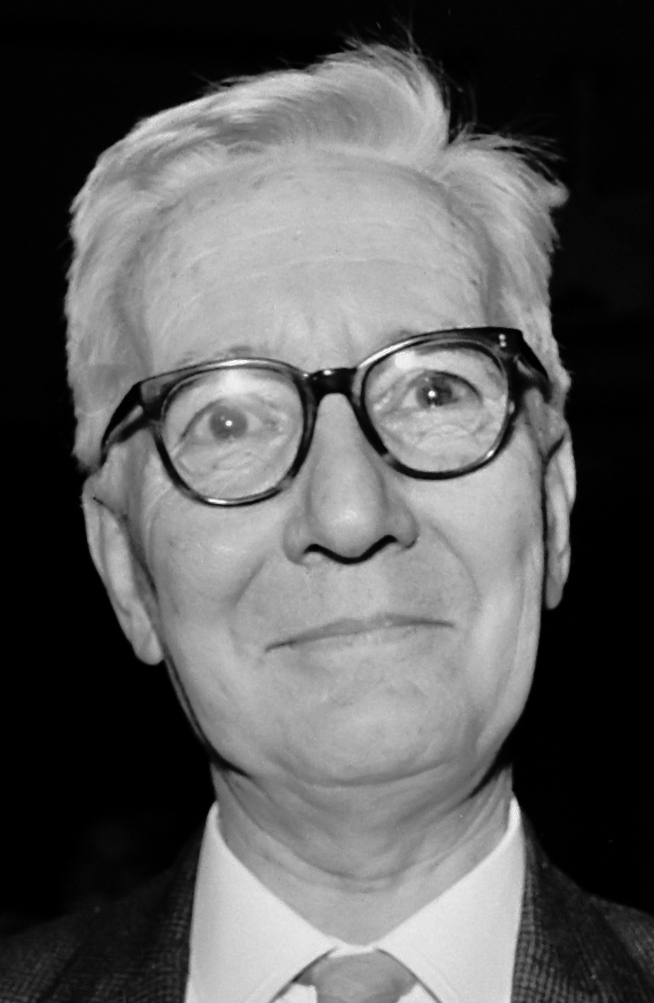
\includegraphics[width=0.36\linewidth]{images/book5/tinbergen.jpg}\hspace{0.04\linewidth}
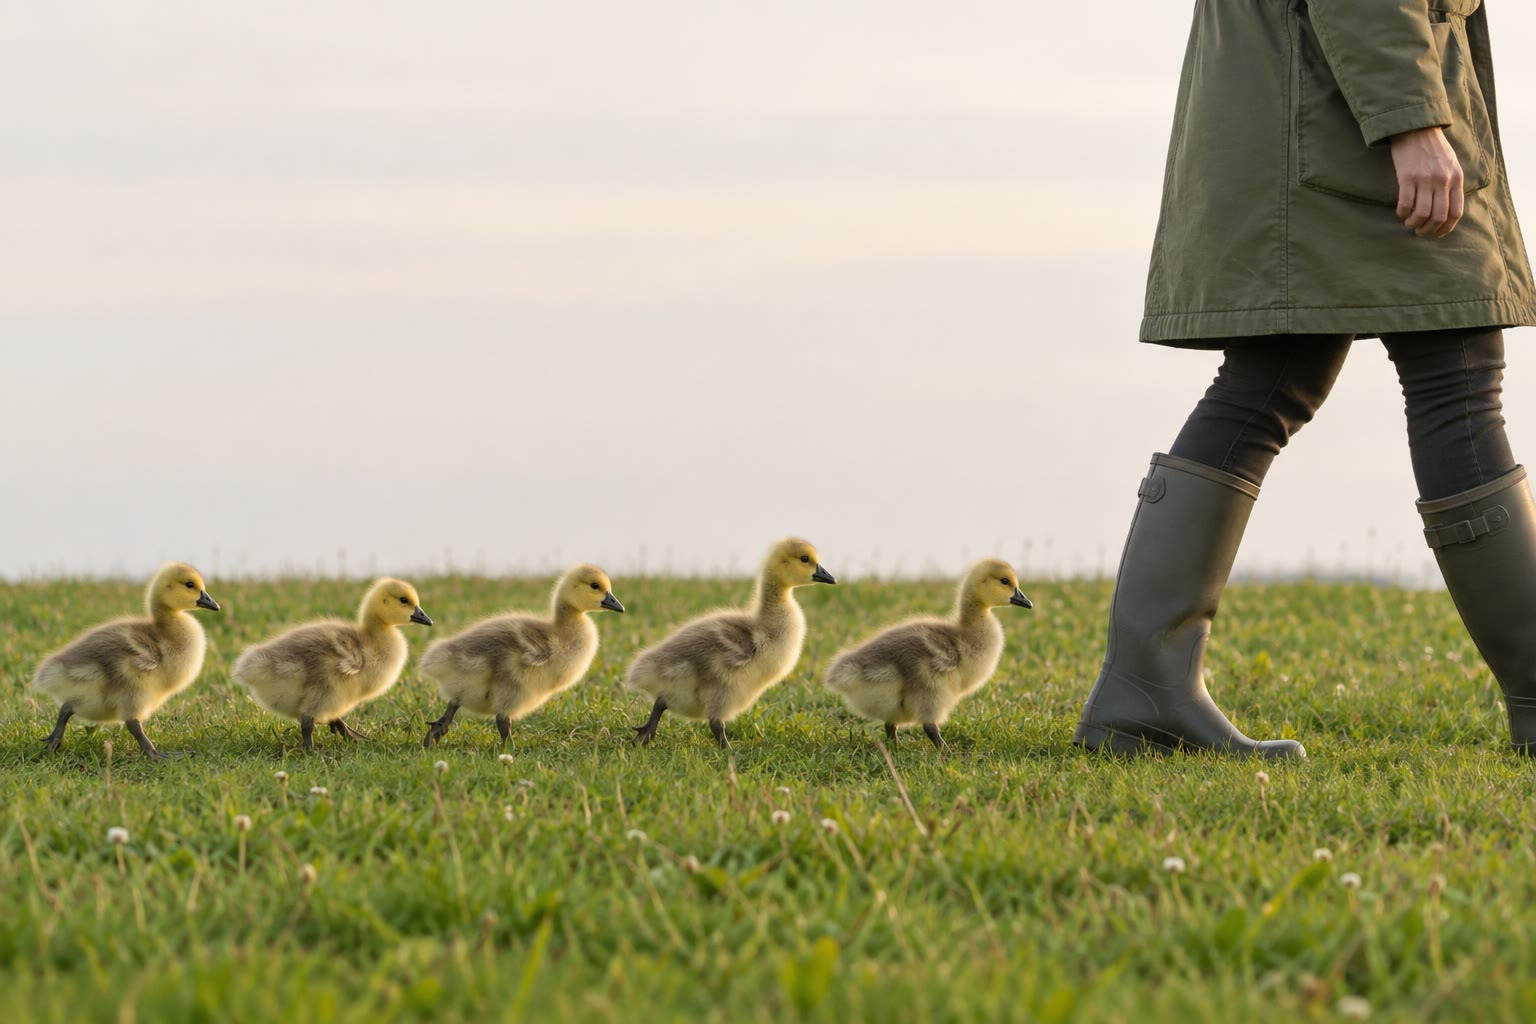
\includegraphics[width=0.52\linewidth]{images/book5/ai/b5-26-goose-imprinting.jpg}

{\small يسارًا: نيكو تينبرغن (1907--1988)، الذي حمل أسئلة
السلوك إلى الميدان وجعلها تجريبية (صورة بعدسة روب ميرمت،
Anefo، 1973، CC0). ويمينًا: فراخ إوز تتبع أول شيء كبير متحرك
رأته، بعد يوم من الفقس، ولم تُقنع بعد ذلك بغيره أبدًا.}
\end{omfigure}

\section{القرار: الارتياد الأمثل}

\begin{theorem}[مبرهنة القيمة الحدية]\label{thm:b3:behavioural-ecology:mvt}
\index{ارتياد أمثل}\index{مبرهنة القيمة الحدية}\index{زمن المكث في الرقعة}\index{عملة}
مرتاد يزور رقعًا من الطعام يفصلها زمن سفر $\tau$. ويكسب في
الرقعة طاقة $g(t)$ بعد زمن $t$، حيث $g$ متزايدة ومقعّرة (إذ
تستنفد الرقعة). فإذا غادر كل رقعة بعد زمن $t$، كان معدل كسبه
على المدى الطويل $R(t) = g(t)/(\tau + t)$، وحقق زمن المكث
$t^{*}$ الذي يعظّمه الشرط
\[
g'(t^{*}) = \frac{g(t^{*})}{\tau + t^{*}} = R(t^{*}) :
\]
أي غادر الرقعة حين يهبط معدل الكسب اللحظي فيها إلى المعدل
الوسطي على الموئل كله، والسفر محسوب (تشارنوف،
1976). والنتائج: أنه كلما طال زمن السفر طال المكث
واستُنفدت كل رقعة استنفادًا أتم؛ وأنه في موئل أغنى
($R$ أعلى) تُغادر كل رقعة أبكر وأقل استنفادًا؛ وأن الرقع كلها
تُغادَر عند المعدل الحدي نفسه مهما تكن جودتها، فتُغادر
الرقعة الفقيرة فورًا تقريبًا والغنية حين
تكون قد نُزلت إلى وسطي الموئل. وعند $g(t) = A(1 -
\mathrm{e}^{-t/T_{0}})$ يصير الشرط $(\tau + t^{*})/T_{0} =
\mathrm{e}^{t^{*}/T_{0}} - 1$، ويُحلّ عدديًا: فعند $\tau = T_{0}$،
$t^{*} \approx 1.15\,T_{0}$؛ وعند $\tau = 4T_{0}$، $t^{*} \approx
2.0\,T_{0}$.
\end{theorem}
\begin{proof}
$R(t) = g(t)/(\tau + t)$؛ و$R'(t) = [g'(t)(\tau + t) - g(t)]/(\tau +
t)^{2} = 0$ يعطي $g'(t^{*}) = g(t^{*})/(\tau + t^{*})$. وهندسيًا:
ارسم $g$ في مقابل $t$ والمبدأ عند $-\tau$؛ فيكون $R(t)$ ميل
المستقيم من $(-\tau, 0)$ إلى $(t, g(t))$، وأعظم ما يكون حيث
يمسّ ذلك المستقيم المنحني --- وهو الشرط. و$\tau$ الأكبر ينقل
المبدأ يسارًا ونقطة التماس يمينًا؛ والموئل الأغنى يزيد ميل
المماس وينقله يسارًا. وأما الأسّي: فيكون $g' = (A/T_{0})
\mathrm{e}^{-t/T_{0}}$ و$g/(\tau + t) = A(1 - \mathrm{e}^{-t/T_{0}})/
(\tau + t)$؛ وبمساواتهما وإعادة الترتيب تنتج المعادلة المذكورة،
وبتعويض $t^{*} = 1.15T_{0}$ عند $\tau = T_{0}$: يسارًا $2.15$، ويمينًا
$\mathrm{e}^{1.15} - 1 = 2.16$.
\end{proof}

\begin{omfigure}
\begin{tikzpicture}
\begin{axis}[
  width=0.68\linewidth, height=5.8cm,
  axis x line=middle, axis y line=left,
  xmin=-4.5, xmax=5, ymin=0, ymax=1.15,
  xlabel={الزمن (بوحدات $T_{0}$)}, ylabel={الطاقة المكتسبة في الرقعة},
  xlabel style={font=\small, at={(axis description cs:0.95,0.0)}, anchor=north}, ylabel style={font=\small},
  tick label style={font=\small}, xtick={-4,-1,0,1.15,2}, xticklabels={$-4T_0$,$-T_0$,0,$1.15$,$2.0$}, ytick={0.5,1}, yticklabels={$0.5A$,$A$},
  clip=false,
]
\addplot[very thick, omDef, domain=0:5, samples=80] {1-exp(-x)};
\draw[thick, omThm] (axis cs:-1,0) -- (axis cs:1.55,1.13);
\draw[thick, omMeth!70!black] (axis cs:-4,0) -- (axis cs:3.5,1.081);
\fill[omThm] (axis cs:1.15,0.6834) circle (2pt); \fill[omMeth!70!black] (axis cs:2,0.8647) circle (2pt);
\draw[dashed, gray] (axis cs:1.15,0) -- (axis cs:1.15,0.6834); \draw[dashed, gray] (axis cs:2,0) -- (axis cs:2,0.8647);
\node[font=\scriptsize, omThm, anchor=north west, align=left] at (axis cs:-4.4,1.1) {سفر قصير، $\tau = T_{0}$:\\غادر عند $t^{*} = 1.15\,T_{0}$،\\والرقعة مستنفدة \qty{68}{\%}};
\node[font=\scriptsize, omMeth!70!black, anchor=north west, align=left] at (axis cs:2.4,0.62) {سفر طويل، $\tau = 4T_{0}$:\\غادر عند $t^{*} = 2.0\,T_{0}$،\\ومستنفدة \qty{86}{\%}};
\node[font=\scriptsize, omDef, anchor=north west] at (axis cs:3.0,0.86) {$g(t) = A(1 - \mathrm{e}^{-t/T_{0}})$};
\node[font=\scriptsize, gray, anchor=south] at (axis cs:-2.5,0.02) {سفر};
\end{axis}
\end{tikzpicture}

{\small \omterm{thm:b3:behavioural-ecology:mvt}{مبرهنة القيمة الحدية} مرسومة. منحني الكسب يفلطح مع
استنفاد الرقعة؛ وميل المستقيم من بداية الرحلة إلى نقطة على
المنحني يساوي معدل الكسب الكلي؛ وأفضل وقت للمغادرة حيث يكون
ذلك المستقيم مماسًّا. والرحلة الأطول تنقل المبدأ يسارًا ونقطة
التماس يمينًا.}
\end{omfigure}

\begin{proof}[شواهد]
ترك كاوي (1977) قراقف كبيرة تصطاد ديدان الوجبة المخبأة في
أكواب مملوءة بنشارة الخشب في قفص، مع التحكم بزمن السفر بين
الأكواب بتركيب أغطية تستغرق إزالتها وقتًا أطول أو أقصر؛
فمكثت الطيور أطول في كل كوب حين كان السفر أبطأ، متتبعةً
تنبؤ المبرهنة، وتجاوزته قليلًا في الاتجاه الذي يفسره حسبان
كلفة السفر الطاقية. والزرازير التي تحمل يرقات الذباب الطويل
إلى فراخها (كاسيلنيك، 1984) أخذت حمولات أكبر من مغذّيات
وُضعت أبعد، وذلك أيضًا كما يقتضي الحل المعظِّم للمعدل لمنحني
تحميل. ولا يبرهن أي من الاختبارين على أن الطيور تحسب
مماسات؛ بل يبيّنان أن الانتخاب أنتج قواعد إبهامية تكون
نتيجتها قريبة من الأمثل.
\end{proof}

\section{المنازعات: نظرية الألعاب}

\begin{proposition}[الصقر والحمامة والاستراتيجية المستقرة تطوريًا]\label{prop:b3:behavioural-ecology:hawk-dove}
\index{نظرية الألعاب}\index{لعبة الصقر والحمامة}\index{استراتيجية مستقرة تطوريًا}\index{انتخاب معتمد على التواتر}
حين يتوقف أفضل سلوك على ما يفعله الآخرون، لا يكون هناك أمثل،
بل \emph{لعبة}. فحيوانان يتنازعان موردًا قيمته $V$؛
و\emph{الصقر} يقاتل حتى يُصاب (بكلفة $C$) أو ينتصر،
و\emph{الحمامة} تستعرض وتنسحب إن هوجمت. ومتوسطات العوائد
\[
\begin{array}{c|cc}
 & \text{vs Hawk} & \text{vs Dove}\\ \hline
\text{Hawk} & (V - C)/2 & V\\
\text{Dove} & 0 & V/2
\end{array}
\]
و\emph{\omterm{prop:b3:behavioural-ecology:hawk-dove}{الاستراتيجية المستقرة تطوريًا}} (ماينارد سميث وبرايس، 1973)
هي التي، متى شاعت، لا يقدر أي بديل نادر على غزوها.
فإذا كان $V > C$، كان الصقر هو المستقرة: فالقتال يؤتي ثمنه
حتى في مواجهة المقاتلين. وإذا كان $V
< C$، لم تكن أي استراتيجية صرفة مستقرة --- إذ تغزو الصقورُ
جمهرةً من الحمائم فتربح كل منازعة، وتغزو الحمائمُ جمهرةً من
الصقور فتتجنب الإصابات --- وتكون المستقرة أن يُلعب الصقر
باحتمال
\[
p^{*} = \frac{V}{C},
\]
أو، بالتكافؤ، جمهرة تكون تلك النسبة فيها صقورًا. وعند
المستقرة تفعل الاستراتيجيتان فعلًا متساويًا، وسطي كل واحدة
$V(1 -
V/C)/2$، وهو أقل من $V/2$ التي كانت جمهرة من الحمائم
ستتقاسمها: فالمنازعة تكلف الجميع، ولا يقدر أحد على تحسين
حاله وحده. والانتخاب هنا \emph{معتمد على التواتر}: إذ تهبط
ملاءمة استراتيجية كلما شاعت، ولذلك تكون منازعات الحيوانات
استعراضًا في معظمها وحربًا أحيانًا، ولذلك يدوم الخليط.
\end{proposition}
\begin{proof}
لتلعب نسبة $p$ الصقر. فالعائد المتوقع للصقر $W_{H} = p(V
- C)/2 + (1 - p)V$؛ وللحمامة $W_{D} = (1 - p)V/2$. و$W_{H} - W_{D} =
p(V - C)/2 + (1 - p)V/2 = [V - pC]/2$، وهو موجب عند $p < V/C$
وسالب فوقه: فتنتشر الصقور إذا كانت نادرة وتُنقّى إذا شاعت،
ويستقر التواتر حيث $W_{H} = W_{D}$، أي عند $p^{*} = V/C$. وأما
استقراره فيتبع من تغيّر الإشارة: فاضطراب $p$ فوق
$p^{*}$ يحابي الحمائم ويُصحَّح، ودونه يحابي الصقور. وإذا كان $V
\ge C$ كان الفرق موجبًا لكل $p \le 1$ وتثبّت الصقر.
والعائد المشترك عند $p^{*}$: $W_{D} = (1 - V/C)V/2$.
\end{proof}

\begin{omfigure}
\begin{tikzpicture}
\begin{axis}[
  width=0.6\linewidth, height=5.4cm,
  axis x line=bottom, axis y line=left,
  xmin=0, xmax=1, ymin=-1, ymax=4.2,
  xlabel={نسبة الصقور $p$}, ylabel={العائد المتوقع},
  xlabel style={font=\small, at={(axis description cs:0.5,-0.12)}, anchor=north}, ylabel style={font=\small},
  tick label style={font=\small}, xtick={0,0.5,1}, xticklabels={0,$p^{*} = V/C$,1}, ytick={0,1,2,4},
  clip=false,
]
\addplot[very thick, omThm, domain=0:1, samples=2] {x*(4-8)/2 + (1-x)*4};
\addplot[very thick, omDef, domain=0:1, samples=2] {(1-x)*4/2};
\draw[dashed, gray] (axis cs:0.5,-1) -- (axis cs:0.5,1);
\fill[black] (axis cs:0.5,1) circle (2pt);
\node[font=\scriptsize, omThm, anchor=north west] at (axis cs:0.5,3.9) {الصقر: $p(V - C)/2 + (1 - p)V$};
\node[font=\scriptsize, omDef, anchor=south west] at (axis cs:0.62,0.9) {الحمامة: $(1 - p)V/2$};
\node[font=\scriptsize, anchor=west, align=left] at (axis cs:0.55,2.6) {$V = 4$، و$C = 8$:\\المستقرة عند $p^{*} = 0.5$،\\والعائد $V(1 - V/C)/2 = 1$};
\draw[->, thick, omThm] (axis cs:0.1,-0.5) -- (axis cs:0.4,-0.5); \draw[->, thick, omDef] (axis cs:0.9,-0.5) -- (axis cs:0.6,-0.5);
\node[font=\tiny, anchor=north] at (axis cs:0.25,-0.55) {تنتشر الصقور}; \node[font=\tiny, anchor=north] at (axis cs:0.75,-0.55) {تنتشر الحمائم};
\end{axis}
\end{tikzpicture}

{\small \omterm{prop:b3:behavioural-ecology:hawk-dove}{لعبة الصقر والحمامة}. حيث يتقاطع خطا العائد، تفعل
الاستراتيجيتان فعلًا متساويًا ولا تقدر إحداهما على الانتشار؛
وعلى أي من الجانبين يدفع الانتخاب التواتر راجعًا. فالخليط
مستقر ويكلف الجميع، وهو ما تبدو عليه منازعات الحيوانات.}
\end{omfigure}

\begin{example}[ألعاب في الميدان]\label{ex:b3:behavioural-ecology:games}
تتنازع ذكور فراشة الخشب المرقّطة بقع الشمس على أرض الغابة:
فالمقيم يربح دائمًا تقريبًا طيرانًا حلزونيًا قصيرًا، وحين
يُخدَع ذكران فيظن كل منهما نفسه مقيمًا يدوم القتال عشرة
أضعاف --- أي عرف (``المقيم يربح'') يحسم المنازعات
رخيصًا، وهو نفسه استراتيجية مستقرة حين يكون القتال مكلفًا
والمورد قليل القيمة. وذكور ذباب الروث تنتظر على فضلات البقر
الإناثَ وتغادر حين يهبط معدل الوصول إلى ما تعرضه فضلة طازجة
--- أي \omterm{thm:b3:behavioural-ecology:mvt}{مبرهنة القيمة الحدية} من جديد، في لعبة تتوقف فيها قيمة
الرقعة على كم منافس يجلس عليها. وزنابير التين، وسحالي
البقعة الجانبية بأنماط ذكورها الثلاثة التي يغلب بعضها بعضًا
دوريًا كالحجر والورقة والمقص، وذكور ``المتسللين'' في السلمون
وشمس الزرقاء، التي تلقّح البيوض باندفاعها من جانب الذكور
الإقليمية التي لا تقدر على قتالها، كلها خلائط محفوظة عند
تواترات تدفع فيها البدائل دفعًا متساويًا. وحرب الاستنزاف ---
حيوانان يستعرضان حتى يستسلم أحدهما، والاستراتيجية المستقرة
أن يثابر المرء زمنًا عشوائيًا مسحوبًا من توزيع أسّي ---
تصف منازعات التحديق في أنواع كثيرة، وتتنبأ، تنبؤًا صحيحًا،
بأن مثابرة الخاسر لا تفشي شيئًا عمّا كان سيدوم.
\end{example}

\section{القرابة: قاعدة هاملتون}

\begin{theorem}[قاعدة هاملتون]\label{thm:b3:behavioural-ecology:hamilton}
\index{قاعدة هاملتون}\index{انتخاب القرابة}\index{قرابة}\index{ملاءمة شاملة}\index{إيثار}\index{أحادية-ثنائية الصيغة}
أليل يجعل حامله يؤدي فعلًا يكلفه $c$ من الخلف ويعطي قريبًا
$b$ من الخلف الإضافي ينتشر إذا كان
\[
r\,b > c ,
\]
حيث $r$ هو \emph{معامل القرابة}: أي احتمال
أن تكون مورّثة في المتلقي نسخةً، بالانحدار، من المورّثة نفسها
في الفاعل --- $1/2$ للوالد والخلف أو للأشقاء،
و$1/4$ لأنصاف الأشقاء والأحفاد وبنات الإخوة وأبنائهم، و$1/8$
لأبناء العمومة من الدرجة الأولى. والمقدار الذي يعظّمه الأليل
هو \emph{\omterm{thm:b3:behavioural-ecology:hamilton}{الملاءمة الشاملة}} لحامله: أي تكاثره هو مضافًا إليه
آثاره في تكاثر أقاربه، كل واحد مرجَّحًا بالمعامل $r$. و\emph{الإيثار}
--- أي سلوك يخفض تكاثر الفاعل ويرفع تكاثر غيره ---
يتطور إذن نحو القرابة، تناسبًا مع درجتها، وتتنبأ
القاعدة بأين ينبغي أن يوجد: في نداءات الإنذار عند إناث
السناجب الأرضية، اللواتي يعشن بين أخواتهن وبناتهن، لا عند
الذكور، الذين يتفرقون؛ وفي حراسة السرقاط، الذي تكون جماعته
أسرة؛ وفي المساعدين عند عش الطيور التي تعين والديها على
تربية إخوتها حين تمتلئ الأقاليم. وفي غشائيات الأجنحة
\emph{\omterm{thm:b3:behavioural-ecology:hamilton}{أحادية-ثنائية الصيغة}} --- ذكورها من بيوض غير ملقحة بطقم
صبغيات واحد، وإناثها بطقمين --- تتشارك الشقيقات ثلاثة
أرباع مورّثاتهن ($r = 3/4$)، أي أكثر مما تتشارك الأم مع
بناتها ($1/2$)، وهو ما اقترحه هاملتون سببًا لنشوء
طوائف الشغالات العقيمة في النمل والنحل والزنابير هناك إحدى
عشرة مرة وفي غيرها لا تكاد تنشأ أبدًا.
\end{theorem}
\begin{proof}
تأمل نسخ الأليل. فحين يؤدي الفاعل الفعل، تخسر نسخه هو $c$ من
الانتقال المتوقع؛ والمتلقي يحمل الأليل باحتمال $r$ فوق وسطي
الجمهرة، فيرفع كسب المتلقي $b$ انتقالَ الأليل بمقدار $rb$
وسطيًا. ويزداد تواتر الأليل حين يكون $rb - c > 0$ (هاملتون،
1964؛ والاشتقاق العام، من التغاير بين النمط الوراثي للفرد
وملاءمته، هو معادلة برايس، وهي مُسلَّم بها
هنا). وأما القرابة: فالوالد ينقل كل مورّثة إلى خلف باحتمال
$1/2$؛ وشقيقان تلقى كل منهما مورّثة معينة من
الوالد نفسه باحتمال $1/2$، وتكون النسخة نفسها باحتمال
$1/2$، والوالدان اثنان: فيكون $r = 2\times\tfrac{1}{2}
\times\tfrac{1}{2} = \tfrac{1}{2}$. وأما الشقيقات أحاديات-ثنائيات
الصيغة: فمن أبيهن الفردي الصيغة يتلقين مورّثات متطابقة
(باحتمال $1$)؛ ومن أمهن نسخًا متطابقة باحتمال $1/2$؛ وبالتوسيط
على الوالدين، $r = (1 + 1/2)/2 = 3/4$.
\end{proof}

\begin{omfigure}
\begin{tikzpicture}[every node/.style={font=\scriptsize}, >=stealth]
  % diploid pedigree
  \node[draw, circle, fill=omDef!30, minimum size=6mm] (m) at (0,3) {}; \node[draw, fill=omDef!30, minimum size=6mm] (f) at (1.6,3) {};
  \node[above, font=\tiny] at (0.8,3.4) {والدان ثنائيا الصيغة};
  \draw[thick] (m) -- (f);
  \node[draw, circle, fill=omThm!40, minimum size=6mm] (a) at (0,1.5) {}; \node[draw, circle, fill=omDef!15, minimum size=6mm] (s) at (1.6,1.5) {};
  \draw[thick] (0.8,3) -- (0.8,2.2) -- (0,2.2) -- (a); \draw[thick] (0.8,2.2) -- (1.6,2.2) -- (s);
  \node[draw, circle, fill=omDef!15, minimum size=6mm] (c) at (1.6,0) {}; \draw[thick] (s) -- (c);
  \node[draw, circle, fill=omDef!15, minimum size=6mm] (o) at (0,0) {}; \draw[thick] (a) -- (o);
  \node[left, omThm, font=\tiny] at (-0.4,1.5) {الفاعل};
  \node[right, font=\tiny] at (1.95,1.5) {شقيق: $r = 1/2$};
  \node[right, font=\tiny] at (1.95,0) {بنت أخ: $r = 1/4$};
  \node[left, font=\tiny] at (-0.4,0) {خلفه هو: $1/2$};
  \node[right, font=\tiny] at (1.95,3) {والد: $r = 1/2$};
  % haplodiploid
  \begin{scope}[shift={(7.2,0)}]
    \node[draw, circle, fill=omDef!30, minimum size=6mm] (q) at (0,3) {}; \node[draw, fill=omMeth!40, minimum size=6mm] (d) at (1.6,3) {};
    \node[above left, font=\tiny] at (0.1,3.3) {ملكة (ثنائية الصيغة)}; \node[above right, font=\tiny] at (1.5,3.3) {ذكر (فردي الصيغة)};
    \draw[thick] (q) -- (d);
    \node[draw, circle, fill=omThm!40, minimum size=6mm] (w) at (0,1.5) {}; \node[draw, circle, fill=omDef!15, minimum size=6mm] (w2) at (1.6,1.5) {};
    \draw[thick] (0.8,3) -- (0.8,2.2) -- (0,2.2) -- (w); \draw[thick] (0.8,2.2) -- (1.6,2.2) -- (w2);
    \node[left, omThm, font=\tiny] at (-0.4,1.5) {شغّالة};
    \node[right, align=left, font=\tiny] at (1.95,1.5) {شقيقة: $r = 3/4$\\(مورّثات الأب متطابقة،\\ومورّثات الأم مشتركة بنسبة $1/2$)};
    \node[draw, circle, fill=omDef!15, minimum size=6mm] (wd) at (0,0) {}; \draw[thick] (w) -- (wd);
    \node[right, font=\tiny] at (0.35,0) {بنتها هي: $1/2$ --- أقل من شقيقة};
  \end{scope}
  \node[below, align=center] at (4.6,-0.9) {قاعدة هاملتون: ساعِد حين $r\,b > c$؛ والشغالة أحادية-ثنائية الصيغة التي تربي شقيقات\\تنقل من مورّثاتها لكل خلف أكثر مما تنقل واحدة تربي بنات};
\end{tikzpicture}

{\small القرابة في ضربين من الأسر. ففي شجرة نسب ثنائية الصيغة
يساوي الشقيق نصف خلف؛ وفي مستعمرة \omterm{thm:b3:behavioural-ecology:hamilton}{أحادية-ثنائية الصيغة} تساوي
الشقيقة أكثر من بنت، وهو ما يميل بالحساب نحو البقاء في
البيت للمساعدة.}
\end{omfigure}

\begin{proof}[شواهد]
راقب شيرمان (1977) سناجب بلدنغ الأرضية ثلاثة صياف
وسجّل من أطلق نداءات الإنذار عند اقتراب المفترسات: فنادت
الإناث اللواتي لهن أقارب قريبون أكثر بكثير من الإناث بلا
أقارب، وأكثر من الذكور، الذين كانوا قد تفرقوا عن مسقط رأسهم
ولا أقارب لهم على مسمع --- فالمنادي جذب انتباه المفترس، ودفع
ثمن ذلك، حين كان هناك أقارب يُنذَرون فقط. وآكلات النحل
البيضاء الجبهة عند إملن تساعد عند العش تناسبًا مع القرابة،
فتختار من الأعشاش المتاحة أعشاش أقرب الأقارب. ووجدت دراسة
كلاتون-بروك الطويلة للسرقاط أن الحراس هم الأفراد جيدو
التغذية الذين لديهم أقل ما يخسرونه، وأن بقاء الجماعة ---
ومن ثم بقاء أقارب الحارس --- يرتفع مع جهد الحراسة؛ غير أن
الكلفة تبيّن أنها أصغر مما افترضته القصة، إذ يكون الحارس
على التل كثيرًا ما أول من يبلغ جحرًا.
\end{proof}

\begin{omfigure}
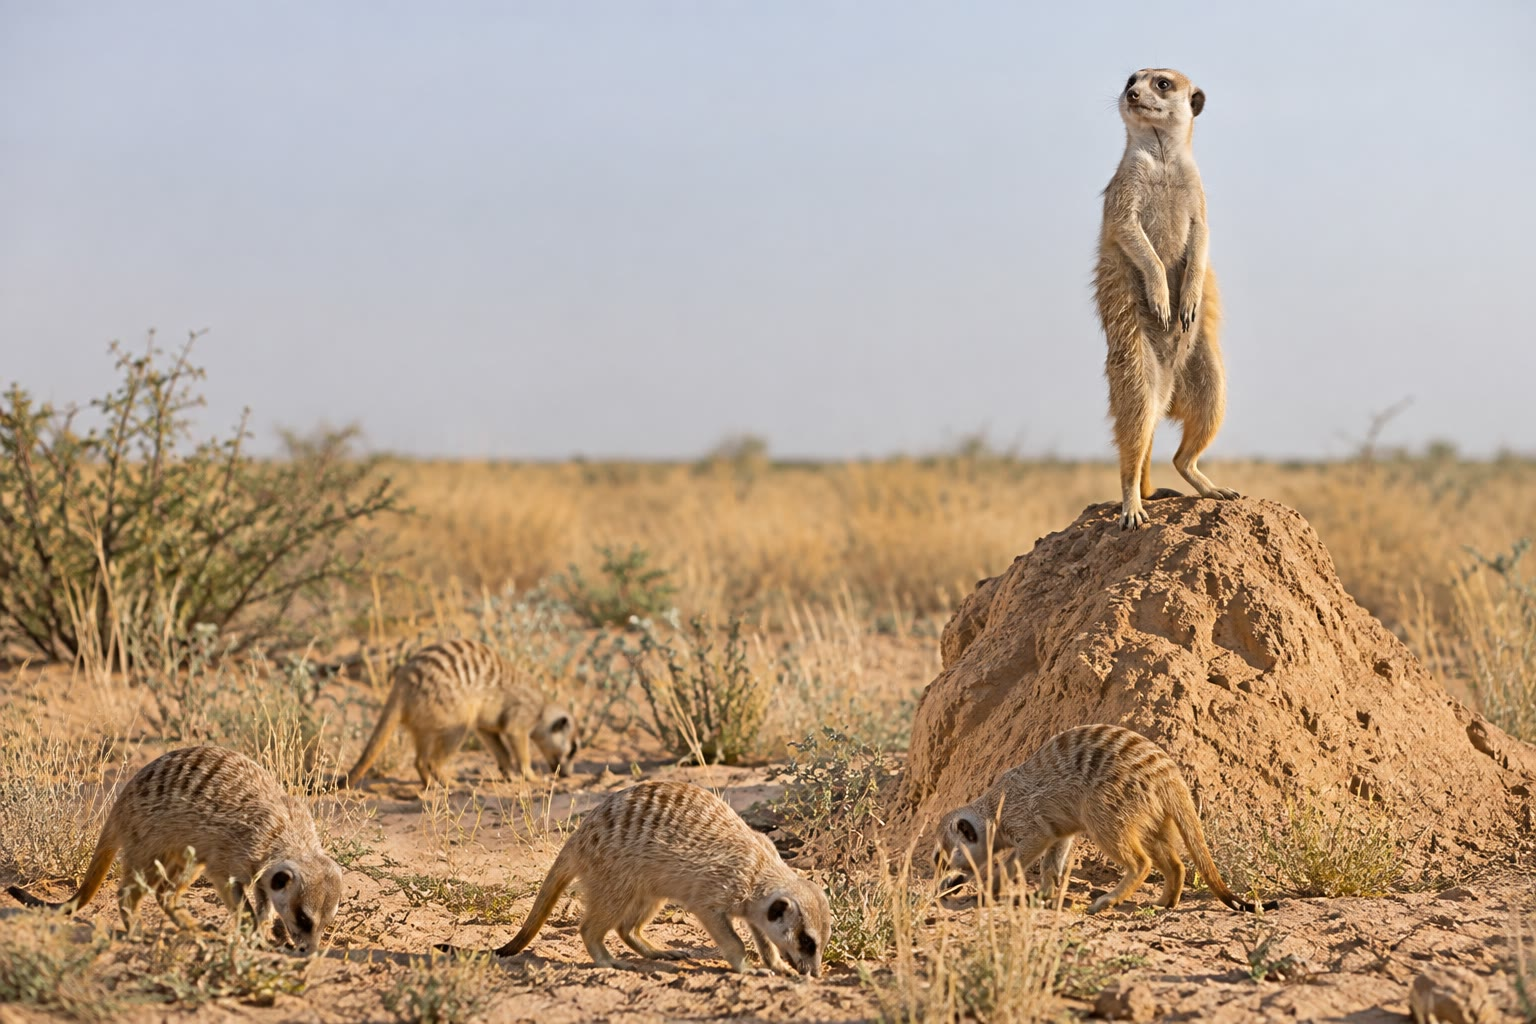
\includegraphics[width=0.46\linewidth]{images/book5/ai/b5-26-meerkat-sentinel.jpg}\hspace{0.04\linewidth}
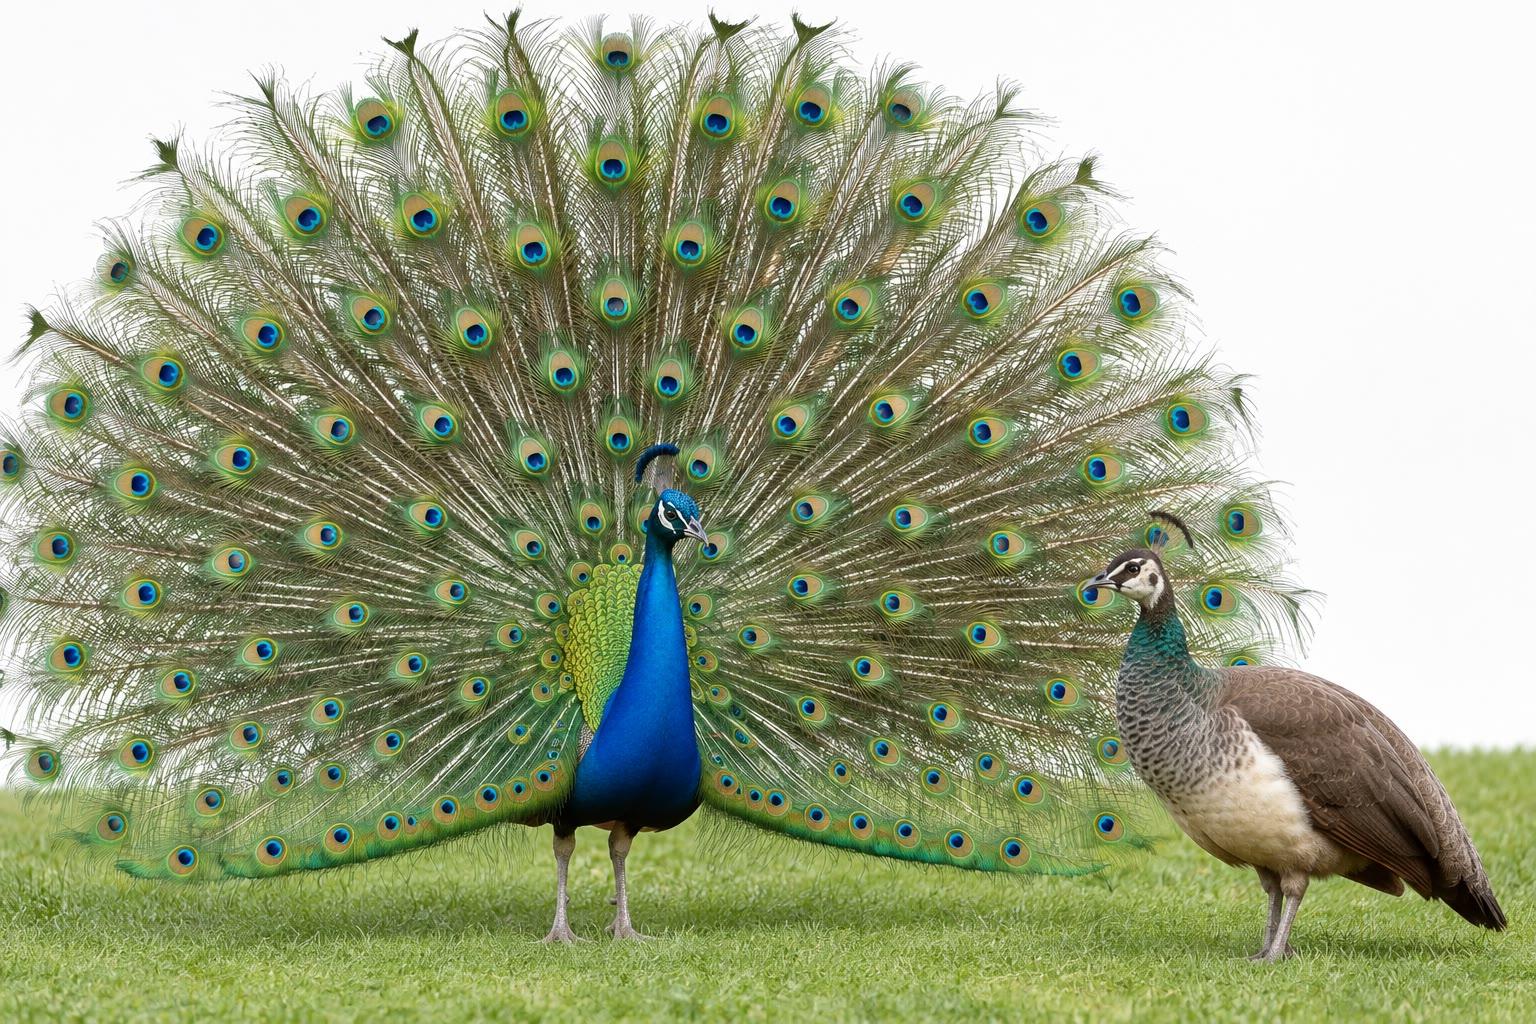
\includegraphics[width=0.46\linewidth]{images/book5/ai/b5-26-peacock-display.jpg}

{\small يسارًا: سرقاط في نوبة حراسة فوق جماعة مرتادة من
أقاربه. ويمينًا: طاووس يستعرض أمام أنثاه --- بنية تكلف حاملها
في الطعام والسرعة ولا تشتري له إلا
انتباهها.}
\end{omfigure}

\section{الأزواج والرسائل}

\begin{definition}[الانتخاب الجنسي]\label{def:b3:behavioural-ecology:sexual-selection}
\index{انتخاب جنسي}\index{ميل بيتمان}\index{انتخاب جامح}\index{مبدأ العائق}\index{مورّثات جيدة}\index{صراع جنسي}
آلية داروين الثانية: الانتخاب على صفات تربح الأزواج لا
البقاء. وجذره تغاير العروس --- فتكاثر الأنثى محدود بالبيوض
التي تقدر على صنعها وتموينها، وتكاثر الذكر بالإناث
اللواتي يقدر على تلقيحهن --- فترتفع ملاءمة الذكر في معظم
الأنواع ارتفاعًا حادًّا مع عدد تزاوجاته ولا تكاد ترتفع ملاءمة
الأنثى (وهو \emph{ميل بيتمان})؛ فتتنافس الذكور على الإناث
وتختار الإناث بين الذكور. والتنافس يعطي القرون والنصال
والأنياب والحجم الكبير ومنازعات القسم السابق. والاختيار يعطي
الزينة، ولها ثلاثة تفسيرات في سبب تفضيل الإناث لها. فأما \emph{الجموح}
عند فيشر: أن تفضيل ذنب أطول قليلًا والذنبَ الأطول انتشرا
معًا، وكل منهما يجعل الآخر مفيدًا، حتى توازن كلفة الذنب في
البقاء كسبَه في التزاوج. و\emph{العائق} عند زهافي: أن زينة
لا يقدر على إنمائها إلا ذكر صحيح \omterm{prop:b3:behavioural-ecology:signals}{إشارة صادقة} على حاله،
وذلك بالضبط لأنها مكلفة --- فالطاووس ذو الذيل الكامل عليه،
بالبرهان، طفيليات أقل. و\emph{المورّثات الجيدة}
و\emph{الفوائد المباشرة}: أن الأنثى تكسب، عبر وراثة خلفها أو
عبر الإقليم والطعام اللذين يوفرهما الذكر.
ومصالح الجنسين تختلف، و\emph{الصراع الجنسي} --- على
تواتر التزاوج، وعلى من يرعى الصغار، وعلى مصير نطاف زوج
سابق --- سباق تسلح يجري داخل نوع واحد: فسائل ذكر
ذبابة الفاكهة المنوي يقصّر عمر الأنثى ويرفع وضعها للبيوض،
وتطوّر الإناث مقاومة.
\end{definition}

\begin{proof}[شواهد]
قصّ أندرسون (1982) ريش ذيول ذكور طيور الأرملة الطويلة الذيل
في كينيا ولصقها: فاجتذبت الذكور التي أُطيلت ذيولها إلى ضعف
طولها الطبيعي أربعة أضعاف الأعشاش الجديدة إلى أقاليمها
مقارنةً بذكور قُصّرت ذيولها، بينما لم تتأثر الشواهد التي
قُصّت ذيولها وأُعيد لصقها بلا تغيير --- أي تفضيل الإناث لذيل
أطول من أي ذيل ينميه ذكر، وهي بصمة تفضيل مُنتخَب أبعد من
الصفة. ووجدت بيتري (1994) أن إناث الطاووس تزاوجت الذكور
التي حملت ذيولها أكثر البقع العينية، وأن فراخ تلك الذكور
نجت نجاةً أفضل في الغابات التي أُطلقت فيها --- أي فائدة
\omterm{def:b3:behavioural-ecology:sexual-selection}{مورّثات جيدة} مقيسة. وعدّ بيتمان (1948) تزاوجات ذباب الفاكهة
الحامل لطفرات واسمة وخلفها فوجد الميل الذي يحمل اسمه:
فنجاح الذكر التكاثري ارتفع خطيًا مع التزاوجات، ونجاح الأنثى
استوى بعد تزاوج واحد.
\end{proof}

\begin{proposition}[الإشارات الصادقة]\label{prop:b3:behavioural-ecology:signals}
\index{تواصل}\index{إشارة صادقة}\index{رقصة الاهتزاز}\index{إشارة مرجعية}
الإشارة فعل يغيّر سلوك المتلقي وتطوّر ليفعل ذلك؛ وهي لا
تستقر إلا إذا أفاد الطرفين، وسطيًا، أن يرسلا وأن يستجيبا.
وحيث تكون مصالحهما مشتركة تقدر الإشارة على أن تكون رخيصة
دقيقة: فإن \emph{\omterm{prop:b3:behavioural-ecology:signals}{رقصة الاهتزاز}} عند نحلة العسل المرتادة (فون
فريش، في أربعينيات القرن العشرين) ترمّز اتجاه مصدر الطعام
زاويةَ شوط الاهتزاز إلى الشاقول --- أي زاوية المصدر إلى الشمس
--- وترمّز بُعده مدةَ الشوط، نحو ثانية لكل
كيلومتر، وتطير المجنَّدات إلى بضع عشرات من الأمتار من
الهدف؛ وقرود الفرفت تعطي نداءات إنذار متمايزة للنمور
والنسور والأفاعي، ويستجيب السامعون استجابةً ملائمة لكل نداء
يُشغَّل من مكبر مخفي --- أي إشارات \emph{مرجعية}. وحيث تتضارب
المصالح، يجب أن تكون الإشارة مكلفة أو غير قابلة للتزوير لتبقى
صادقة --- كزئير أيل أحمر، الذي لا يقدر على إدامة معدله إلا
أيل لائق؛ وكحجم نقيق ضفدع، الذي يحدده جسمه؛ وكزينة الفقرة
السابقة --- وإلا استُغلت: فيراعات جنس تحاكي
ومضات إناث جنس آخر لتأكل الذكور التي تأتي، ويفوق تسوّل فراخ
الوقواق تسوّل فراخ المضيف نفسه. فنظرية الإشارة تتنبأ
بصورة الإشارة من العلاقة بين الطرفين: رخيصة
مخبِرة بين الأقارب والأزواج الذين تتطابق مصالحهم، ومكلفة
مطقّسة بين المتنافسين، وسباق تسلح بين المفترس والفريسة.
\end{proposition}
\admitted

\begin{omfigure}
\begin{tikzpicture}[every node/.style={font=\scriptsize}, >=stealth]
  % field view
  \node[above] at (0,3.2) {في الميدان};
  \draw[->, thick, gray] (0,0) -- (0,2.6) node[above, font=\tiny] {نحو الشمس};
  \fill[omDef!60] (0,0) circle (0.12); \node[below, font=\tiny] at (0,-0.2) {الخلية};
  \draw[->, very thick, omThm] (0,0) -- ({2.4*sin(40)},{2.4*cos(40)}); \node[right, font=\tiny, omThm] at ({2.4*sin(40)},{2.4*cos(40)}) {الطعام، \qty{1}{km}};
  \draw[omThm] (0,1.0) arc[start angle=90, end angle=50, radius=1.0]; \node[font=\tiny, omThm] at (0.55,1.25) {$40^{\circ}$};
  % comb view
  \begin{scope}[shift={(6.2,0)}]
    \node[above] at (0,3.2) {على القرص العمودي};
    \draw[very thick, gray!60] (-1.8,-0.4) rectangle (1.8,3.0);
    \draw[->, thick, gray] (0,0) -- (0,2.6) node[above, font=\tiny] {إلى أعلى (= الشمس)};
    \draw[->, very thick, omThm] (0,0) -- ({1.6*sin(40)},{1.6*cos(40)}); \node[below, align=center, font=\tiny, omThm] at (0,-0.5) {شوط الاهتزاز: $40^{\circ}$ عن الشاقول؛\\ومدته $\approx \qty{1}{s}$ لكل كيلومتر};
    \draw[omThm, dashed] ({1.6*sin(40)},{1.6*cos(40)}) .. controls (1.3,0.4) and (0.5,-0.3) .. (0,0);
    \draw[omThm, dashed] ({1.6*sin(40)},{1.6*cos(40)}) .. controls (-0.2,1.2) and (-0.6,0.3) .. (0,0);
    \draw[omThm] (0,0.8) arc[start angle=90, end angle=50, radius=0.8]; \node[font=\tiny, omThm] at (0.45,1.0) {$40^{\circ}$};
  \end{scope}
  \node[right, align=left] at (9.2,1.3) {شفرة رمزية: الجاذبية\\تنوب عن الشمس، والزمن\\عن المسافة؛ وتصل المجنَّدات\\في حدود عشرات الأمتار};
\end{tikzpicture}

{\small \omterm{prop:b3:behavioural-ecology:signals}{رقصة الاهتزاز}. زاوية الشوط إلى الشاقول هي زاوية
الطعام إلى الشمس؛ وطول الشوط هو المسافة. وإشارة بهذا الرخص
وبهذه الدقة ممكنة لأن الراقصة وجمهورها شقيقات لهن المصلحة
نفسها.}
\end{omfigure}

\begin{omfigure}
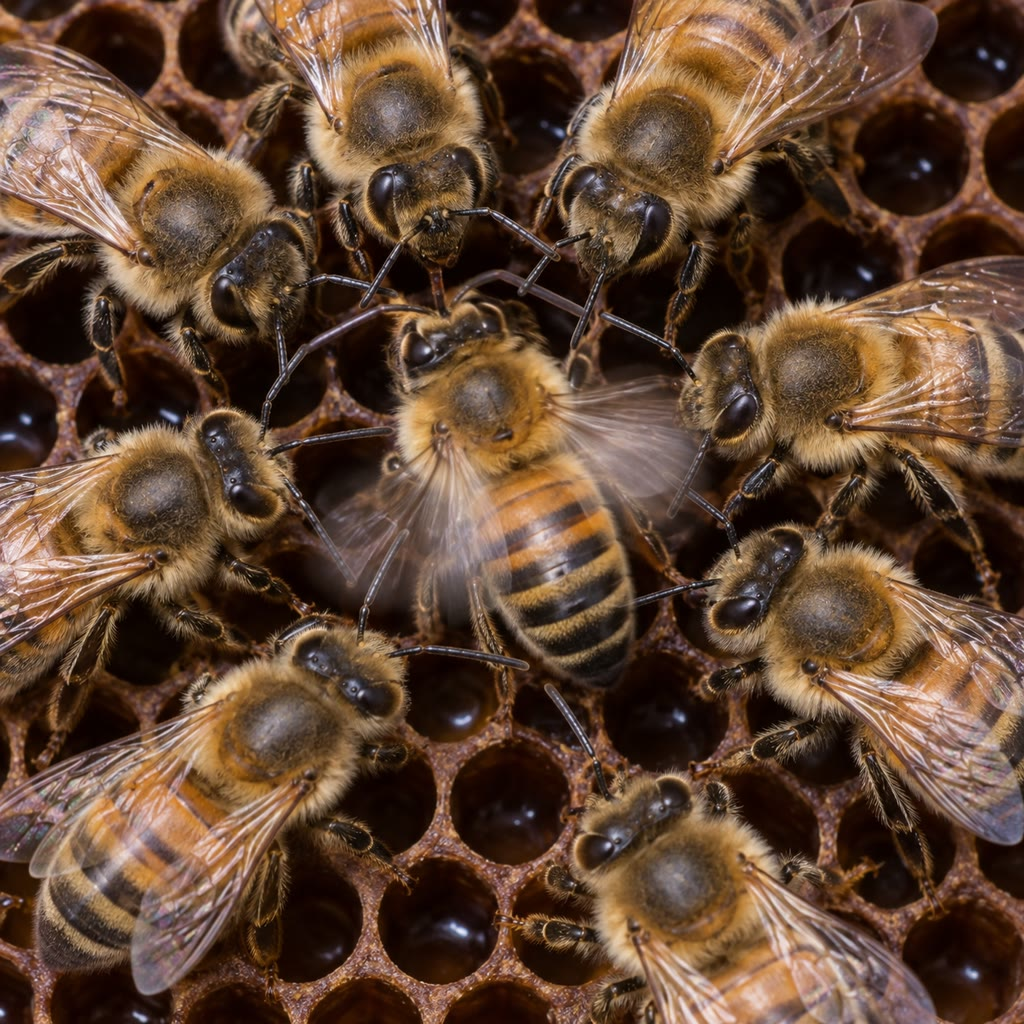
\includegraphics[width=0.4\linewidth]{images/book5/ai/b5-26-bee-dance.jpg}

{\small مرتادة ترقص على القرص، وتحيط بها شغالات يقرأن زاوية
شوطها وإيقاعه.}
\end{omfigure}

\begin{remark}[لماذا تبدو الحيوانات كأنها تحسب]\label{rem:b3:behavioural-ecology:remark}
القرقف الكبير لا يشتق $g(t)/(\tau + t)$، والسرقاط لا يحسب
$r$، وأنثى الطاووس لم تسمع قط بعائق. وإنما يحمل كل واحد
قواعد --- غادِر حين تبطؤ الاصطيادات، ونادِ حين تكون الجماعة
أسرة، وفضّل الأبهى --- شكّلها الانتخاب لأن
الحيوانات التي تتبعها تركت خلفًا أكثر؛ والرياضيات رياضياتنا،
طريقةٌ لسؤال ما الذي يجب أن تحققه القواعد ليكون الأمر كذلك،
ولتنبؤ السلوك في مواقف لم تلقها الحيوانات قط. وحين تخفق
التنبؤات --- إذ يمكث القرقف طويلًا، وتكون كلفة الحارس
أصغر مما افتُرض --- يكون الإخفاق مخبِرًا: فقد أُخطئت عملة، أو
فات قيد، أو أُسيء عدّ قريب. والموضوع
حوار عقدًا بعد عقد بين دفتر ميداني
وسطر من الجبر، وتبقى \omterm{def:b3:behavioural-ecology:tinbergen}{أسئلة تينبرغن الأربعة}
إطارًا لكليهما.
\end{remark}

\section{تمارين}

\begin{exercise}[$\star$]\label{exo:b3:behavioural-ecology:1}
اذكر \omterm{def:b3:behavioural-ecology:tinbergen}{أسئلة تينبرغن الأربعة} وأجب عن كل واحد، في جملة، \omterm{prop:b3:behavioural-ecology:signals}{لرقصة
الاهتزاز}.
\end{exercise}

\begin{exercise}[$\star$]\label{exo:b3:behavioural-ecology:2}
ما \omterm{def:b3:behavioural-ecology:tinbergen}{نمط الفعل الثابت} وما \omterm{def:b3:behavioural-ecology:tinbergen}{المنبّه الإشاري}؟ اذكر مثالين واشرح
ماذا أظهرت العصا ``فوق السوية'' بأشرطتها الحمر الثلاثة.
\end{exercise}

\begin{exercise}[$\star$]\label{exo:b3:behavioural-ecology:3}
بالكلام، ماذا تقول \omterm{thm:b3:behavioural-ecology:mvt}{مبرهنة القيمة الحدية}، وبماذا تتنبأ عن
استعمال الرقع حين يتضاعف زمن السفر؟
\end{exercise}

\begin{exercise}[$\star$]\label{exo:b3:behavioural-ecology:4}
عرّف \omterm{prop:b3:behavioural-ecology:hawk-dove}{الاستراتيجية المستقرة تطوريًا}. ولماذا لا تكون جمهرة من
الحمائم الصرفة كذلك، ولماذا يكلف خليط الصقر والحمامة الجميع؟
\end{exercise}

\begin{exercise}[$\star\star$]\label{exo:b3:behavioural-ecology:5}
الصقر والحمامة عند $V = 6$ و$C = 10$: احسب $p^{*}$، وعائد كل
استراتيجية عند المستقرة، والعائد الذي كانت ستحصل عليه جمهرة
من الحمائم كلها. وأعد ذلك عند $V = 12$ و$C = 10$.
\end{exercise}

\begin{exercise}[$\star\star$]\label{exo:b3:behavioural-ecology:6}
دالة كسب $g(t) = A(1 - \mathrm{e}^{-t/T_{0}})$ عند $T_{0} =
\qty{2}{min}$. جِد $t^{*}$ عند $\tau = 2$ و$\tau = 8$ دقائق (استعمل
قيم الفصل)، ونسبة كل رقعة المستهلكة، والمعدل الطويل المدى $R$
كنسبة من $A$ في الدقيقة.
\end{exercise}

\begin{exercise}[$\star\star$]\label{exo:b3:behavioural-ecology:7}
احسب $r$ بين: أنصاف الأشقاء؛ والجد والحفيد؛ وأبناء العمومة من
الدرجة الأولى؛ وشغّالة \omterm{thm:b3:behavioural-ecology:hamilton}{أحادية-ثنائية الصيغة} وأخيها؛ وملكة
\omterm{thm:b3:behavioural-ecology:hamilton}{أحادية-ثنائية الصيغة} وابنها. اشرح الأخيرين.
\end{exercise}

\begin{exercise}[$\star\star$]\label{exo:b3:behavioural-ecology:8}
نداء إنذار يكلف المنادي احتمال موت قدره \qty{2}{\%} وينقذ
كل واحد من $n$ قريبًا مجاورًا من احتمال قدره \qty{1}{\%}. فعند
أي $n$ تحابي \omterm{thm:b3:behavioural-ecology:hamilton}{قاعدة هاملتون} النداء إذا كان الأقارب أشقاء؟
وبنات إخوة؟ وغير أقارب؟
\end{exercise}

\begin{exercise}[$\star\star$]\label{exo:b3:behavioural-ecology:9}
ذيل طائر الأرملة \qty{50}{cm}؛ وإذا أُطيل إلى \qty{75}{cm}
اجتذب ضعف الأعشاش، وإذا قُصّر إلى \qty{25}{cm} نصفها. فإذا هبط
البقاء \qty{20}{\%} لكل \qty{25}{cm} تُضاف، فأي ذيل يعظّم
جداء التزاوجات والبقاء، ولماذا قد يكون الذيل الطبيعي أقصر
من ذلك؟
\end{exercise}

\begin{exercise}[$\star\star\star$]\label{exo:b3:behavioural-ecology:10}
أضف استراتيجية ثالثة، هي المُقتَصّ، الذي يستعرض كالحمامة لكن
يردّ إن هوجم. اكتب عوائده في مواجهة الصقر والحمامة
ونفسه (ففي مواجهة الصقر يقاتل: $(V - C)/2$؛ وفي مواجهة
الحمامة والمقتَصّ يتقاسم: $V/2$). بيّن أن جمهرة من المقتصّين
لا تقدر الصقور على غزوها حين $V < C$، وناقش هل تقدر الحمائم
على التسرب إليها.
\end{exercise}

\begin{exercise}[$\star\star\star$]\label{exo:b3:behavioural-ecology:11}
في حرب استنزاف، يثابر كل متنازع زمنًا مسحوبًا من
توزيع؛ والاستراتيجية المستقرة أسّية وسطيها $V/$(الكلفة في وحدة
الزمن). اشرح لماذا لا يقدر زمن مثابرة ثابت على أن يكون
مستقرًا، ولماذا يجعل التوزيع الأسّي المثابرةَ المستقبلية
المتوقعة لخصم لا يزال يستعرض مستقلةً عن مدة استعراضه
السابقة.
\end{exercise}

\begin{exercise}[$\star\star\star$]\label{exo:b3:behavioural-ecology:12}
تتنبأ حجة هاملتون في \omterm{thm:b3:behavioural-ecology:hamilton}{أحادية-ثنائية الصيغة} بأن تفضّل الشغالات
تربية الشقيقات ($r = 3/4$) على الإخوة ($r = 1/4$)، بينما تقدّر
الملكة الأبناء والبنات تقديرًا متساويًا. تنبأ بنسبة الجنسين في
التكاثريات التي ينبغي أن تنتجها مستعمرة إذا تحكمت الشغالات
بها، وإذا تحكمت الملكة؛ وقل ماذا وجد تريفرز وهير، وماذا تفعل
بالحجة ملكةٌ تتزاوج بعدة ذكور.
\end{exercise}

\section{مسألة: حساب الحارس}

\begin{problem}[{مسألة نهاية الأسبوع --- يوم في جماعة سرقاط
يُجرى إيكولوجيا سلوكية: أزمنة الرقع في مبرهنة القيمة الحدية،
ومنازعات لعبة الصقر والحمامة واستراتيجيتها المستقرة، ومحاسبة
القرابة في نوبة الحراسة وفي خلية أحادية-ثنائية الصيغة، وكلفة
زينة، وتُختم بزمن المكث في الرقعة، وبتواتر الصقور، وبعتبة
هاملتون للحارس}]
\label{pb:b3:behavioural-ecology:1}
المعطيات: رقع ارتياد عند $g(t) = A(1 - \mathrm{e}^{-t/T_{0}})$، و$T_{0}
= \qty{3}{min}$، و$A = \qty{60}{kJ}$؛ والسفر بين الرقع $\tau =
\qty{3}{min}$ (موئل كثيف) أو \qty{12}{min} (متناثر). ومنازعات على
جحر: $V = 10$، و$C = 30$ (بوحدات الملاءمة). والحارس: نوبة ساعة
تكلف الحارس $c = 0.03$ من مكافئات الخلف (تغذية ضائعة،
وتعرّض)؛ وهي تخفض خطر الافتراس على كل رفيق، بما يساوي $b = 0.01$
من مكافئات الخلف لكل واحد؛ وفي الجماعة $n$ فردًا بقرابة وسطية
$\bar r$. والخلية: تقدر شغّالة على تربية $k$ شقيقة أو $k$
بنت لها بالجهد نفسه. والزينة: طول ذيل $L$ يعطي تزاوجات
$m(L) = L/20$ وبقاءً $s(L) = 1 - (L/100)^{2}$، و$L$ بالسنتيمتر.

\medskip
\noindent\textbf{الجزء الأول --- الرقع.}
\begin{enumerate}
  \item اكتب المعدل الطويل المدى $R(t)$ وشرط القيمة الحدية
        لهذه الدالة $g$.
  \item بيّن أن الشرط يؤول إلى $(\tau + t)/T_{0} = \mathrm{e}^{t/T_{0}}
        - 1$، وحلّه عند $\tau = T_{0}$ (جرّب $t = 1.15\,T_{0}$).
  \item حُلّه عند $\tau = 4T_{0}$ (جرّب $t = 2.0\,T_{0}$).
  \item لكل حالة: زمن المكث بالدقائق، والطاقة في كل رقعة،
        ونسبة الرقعة المستهلكة، والمعدل $R$ بوحدة kJ/min.
  \item قاعدة إبهامية: ``غادِر بعد \qty{5}{min} ثابتة''. احسب
        $R$ للموئلين وقارنه بالأمثل. فهل القاعدة كافية؟
  \item وقاعدة أخرى: ``غادِر حين تمر \qty{20}{s} بلا
        اصطياد''. اشرح لماذا تقارب قاعدة زمن التخلي هذه
        المبرهنة، وفي أي اتجاه تخفق حين تختلف الرقع في الغنى.
\end{enumerate}

\medskip
\noindent\textbf{الجزء الثاني --- المنازعات.}
\begin{enumerate}[resume]
  \item اكتب مصفوفة العوائد واحسب $p^{*}$.
  \item العائد للصقر وللحمامة عند $p = 0.1$، و$p = p^{*}$، و$p =
        0.6$؛ وأي استراتيجية تنتشر في كل حالة؟
  \item العائد عند المستقرة؛ وقارنه بعائد الحمائم كلها. فكم
        تخسر الجمهرة في كل منازعة بسبب إمكان القتال؟
  \item جفاف يرفع $V$ إلى $40$ (إذ تندر الجحور). فما المستقرة
        الجديدة؟ وبماذا يتنبأ ذلك عن القتال في السنين العجاف؟
  \item البرجوازي: ``صقرٌ إن كنت مقيمًا، وحمامةٌ إن كنت
        دخيلًا''، وكل دور نصف الوقت. وعائده في مواجهة نفسه
        $V/2$ بلا قتال. بيّن أن الصقور لا تقدر على غزو جمهرة
        برجوازية حين $V
        < C$، واشرح فراشة الخشب المرقّطة.
  \item اشرح في جملة لماذا يحكم هذا السلوك الاعتمادُ على
        التواتر لا أمثلُ ما.
\end{enumerate}

\medskip
\noindent\textbf{الجزء الثالث --- القرابة.}
\begin{enumerate}[resume]
  \item \omterm{thm:b3:behavioural-ecology:hamilton}{قاعدة هاملتون} للحارس: الشرط على $n\bar r$. فعند أي
        $n\bar r$ تؤتي النوبة ثمنها؟
  \item جماعة من $n = 8$ أشقاء ($\bar r = 1/2$): فهل تؤتي
        ثمنها؟ وجماعة من 8 حيوانات غير قريبة؟ وجماعة من 8
        أنصاف أشقاء؟
  \item الحارس جيد التغذية، فتهبط $c$ عنده إلى $0.01$. فما
        العتبة الآن؟ ولماذا يتنبأ ذلك بأن الحراس هم الأفراد
        جيدو التغذية؟
  \item الخلية: قيمة \omterm{thm:b3:behavioural-ecology:hamilton}{الملاءمة الشاملة} لعدد $k$ من الشقيقات في مقابل
        $k$ بنت. فأيهما ينبغي أن تفضّل الشغّالة، وبأي نسبة؟
  \item تزاوجت الملكة ثلاثة ذكور بالتساوي: فما متوسط قرابة
        الشغالات لشقيقاتهن؟ وهل يبقى التفضيل؟
  \item اشرح لماذا لا تقتضي \omterm{thm:b3:behavioural-ecology:hamilton}{قاعدة هاملتون} أن يتعرف الفاعل
        قرابته، وأي قاعدة إبهامية قد يستعملها سنجاب أرضي فعلًا.
\end{enumerate}

\medskip
\noindent\textbf{الجزء الرابع --- الزينة.}
\begin{enumerate}[resume]
  \item الملاءمة $W(L) = m(L)\,s(L)$. احسب $W$ عند $L = 20$، و$40$، و$60$،
        و$80$.
  \item جِد $L$ الذي يعظّم $W$ تحليليًا، وقيمة $W$ عنده.
  \item تشتد كلفة البقاء إلى $s = 1 - (L/70)^{2}$ (إذ يصل
        مفترس). فما الأمثل الجديد؟ وفي أي اتجاه، ولماذا يتنبأ
        ذلك بأن تطور الذيل يتتبع الافتراس؟
  \item ضاعفت تجربة أندرسون الذيول إلى \qty{75}{cm} وضاعفت
        الأعشاش. فهل يتسق تفضيل الإناث لذيول أطول ``فوق
        الأمثل'' مع تفسير الجموح، أم مع تفسير العائق، أم مع
        الاثنين؟
  \item لماذا لا تكون زينة رخيصة إشارةً صادقة، وكيف تجعلها
        الكلفة في السؤال~21 كذلك؟
  \item ميول بيتمان: يكسب الذكور $0.8$ من الخلف لكل تزاوج
        إضافي، والإناث $0.1$. اشرح في فقرة واحدة كيف يولّد هذا
        اللاتناظر منازعاتِ الجزء~الثاني وزينةَ الجزء~الرابع
        معًا.
  \item لخّص: قيمة $t^{*}$ في الموئل الكثيف (السؤال~4)،
        وقيمة $p^{*}$ (السؤال~7)، وعتبة الحارس $n\bar r$
        (السؤال~13).
\end{enumerate}
\end{problem}
